% !TEX encoding = UTF-8 Unicode
% LaTeX file for resume 
% This file uses the resume document class (res.cls)

\documentclass{res} 
\usepackage{fontspec}
\usepackage{xeCJK}
\usepackage{listings}
\usepackage[autostyle]{csquotes} 
\usepackage{hyperref}
\lstset{language=C,
numberstyle=\footnotesize,
basicstyle=\ttfamily\footnotesize,
numbers=left,
stepnumber=1,
frame=shadowbox,
breaklines=true}
\setCJKmainfont{STHeiti} % chinese type
%\setCJKmainfont{BiauKai}
%\usepackage{helvetica} % uses helvetica postscript font (download helvetica.sty)
%\usepackage{newcent}   % uses new century schoolbook postscript font 
\setlength{\textheight}{9.5in} % increase text height to fit on 1-page 
\usepackage{enumitem}

\XeTeXlinebreakskip = 0pt plus 1pt 

\begin{document} 


\name{\LARGE Real Time System Project2 Report}     % the \\[12pt] adds a blank
				        % line after name
\address{\\R03922106 蔡佑隆 unzledick@yahoo.com.tw\\ R04922067 楊翔雲 morris821028@gmail.com}

\begin{resume}

\vspace*{.1in} \noindent {\large \bfseries 作業描述}

修改 linux kernel,並且增加 Weighted Round-Robin scheduling 和 Shortest Job First scheduling。

\vspace*{.1in} \noindent {\large \bfseries 系統環境}

\begin{itemize}
	\item Ubuntu 14.04.3 LTS
	\item qemu
\end{itemize}


\vspace*{.1in} \noindent {\large \bfseries 環境安裝}

參閱附錄

\vspace*{.1in} \noindent {\large \bfseries 修改檔案列表}

\begin{lstlisting}[frame=single]
.
├── README.md
├── arch
│   └── x86
│       ├── include
│       │   └── asm
│       │       ├── unistd_32.h
│       │       └── unistd_64.h
│       └── kernel
│           └── syscall_table_32.S
├── include
│   └── linux
│       ├── sched.h
│       └── syscalls.h
└── kernel
    ├── sched.c
    ├── sched_fair.c
    ├── sched_rt.c
    └── sched_weighted_rr.c
\end{lstlisting}

特別注意到,若編譯環境為 64-bit 則需要額外修改 \lstinline{arch/x86/include/asm/unistd_64.h} 複製 \lstinline{arch/x86/include/asm/unistd_32.h} 增加的 syscall。 同理,增加自己定義的 syscall 時,需要修改 \lstinline{arch/x86} 下的那三個檔案 (如果發現編譯 kernel 時,出現 \lstinline{WARNING: syscall NOT IMPLEMENTION.} 大多數都是這個造成)。



在 \lstinline{include/linux/sched.h} 中,增加 task member 提供接下來針對 task 操作需要的參數,特別的是在 \lstinline{struct sched_rt_entity;} 中,相較於一般資料結構的寫法,linux 採用倒過來將節點訊息放在資料內部中,利用 \lstinline{#define container_of(ptr, type, member)} 取得物件訊息,預計是這種特別寫法可解決 task 在數個 scheduler 中轉換。

因為 syscall 的方式設定 task 的 weighted round-robin,增加一個全區變數 \lstinline{extern int weighted_rr_time_slice;},每一次 syscall 去設定這一個全區變數值,然後 task create 後,直接利用被修改全區變數作為這一個 task weight round-robin。若要特別針對 task 設定 weighted round-robin,在 create 前都要呼叫一次 syscall。

\begin{lstlisting}[frame=single]
struct sched_rt_entity {
    ...
    //+ RTS Proj2: weighted_rr
    struct list_head weighted_rr_list_item;
    ...
};
...
struct task_struct {
    ...
    //+ RTS Proj2: weighted_rr
    unsigned int task_time_slice;
    //+ RTS Proj2: weighted_rr_prio
    unsigned int weighted_time_slice;
    ...
};
...
//+ RTS Proj2: weighted_rr
extern int weighted_rr_time_slice;
\end{lstlisting}

\vspace*{.1in} \noindent {\large \bfseries sched\_x Source Code}

\begin{itemize}
	\item	
	\lstinline{enqueue_task_weighted_rr(struct rq *rq, struct task_struct *p, int wakeup, bool b)}
	\begin{itemize}
		\item Weighted round-robin \\
	函數將會給予 task 和 rq,將 task 根據 rq 的資料結構重新將 task 放入。若按照 Weighted Round-Robin \lstinline{list} 結構,直接模擬 queue 即可,由於 linux 提供 list 本身為雙向串列,直接加入尾端只需要 $\mathcal{O}(1)$ 時間。並且運行 \lstinline{rq->weighted_rr.nr_running++;} 增加 rq 中的計數,隨後用來在回報該 scheduler 中有沒有存在 task 需要運行,方便在 $\mathcal{O}(1)$ 時間內完成,由於 Weighted round-robin 只需要確認 list 是否為空,那麼也可以利用 linux 提供的 \lstinline{list_empty()} 確認。
		\item Shortest Job First \\
		與 Weighted round-robin 類似,利用 list 做插入排序,可以在最慘 $\mathcal{O}(n)$ 時間內維護一個優先權由高至低的 list。需要 task 時,直接將串列的首元素移除。
	\end{itemize}
	
	\item
	\lstinline{dequeue_task_weighted_rr(struct rq *rq, struct task_struct *p, int sleep)} \\
	\begin{itemize}
		\item Both Weighted round-robin and Shortest Job First \\
		當 task 完成任務時,都要呼叫 \lstinline{update_curr_weighted_rr} 進行統計運行多久,並且更新與 task 相關的排程權重。接著將 task 從 rq 串列中移除,並且更新 scheduler 的 task 計數 (\lstinline{rq->weighted_rr.nr_running--;})。時間複雜度 $\mathcal{O}(1)$
	\end{itemize}
	
	\item
	\lstinline{requeue_task_weighted_rr(struct rq *rq, struct task_struct *p)} \\
	\begin{itemize}
		\item Weighted round-robin \\
		將一個 task 出列,在 Weighted round-robin 只需要直接對 task p 底下的 \lstinline{weighted_rr_list_item} 移到串列最尾端,由於採用雙向串列,直接跟 rq 取得 list head (linux list 的 head 是不存放任何資訊) 直接加入尾端即可。時間複雜度 $\mathcal{O}(1)$
		\item Shortest Job First \\
		在最短工作優先排程中,由於 task priority 會變動,不方便確定執行過一陣子的 task 要移動到哪裡,最簡單的實作方式採用 \lstinline{dequeue} 後再一次 \lstinline{enqueue}。時間複雜度 $\mathcal{O}(n)$
	\end{itemize}
	
	\item
	\lstinline{yield_task_weighted_rr(struct rq)} \\
	\begin{itemize}
		\item Both Weighted round-robin and Shortest Job First\\
		直接運行 requeue 即可。
	\end{itemize}
	
	\item
	\lstinline{pick_next_task_weighted_rr(struct rq *rq)}\\
	\begin{itemize}
		\item Both Weighted round-robin and Shortest Job First\\
		當最上層分配一段時間給 scheduler rq 運行,會調用這個函數,拿取要執行的 task,但並不用將其移除串列,並執行  \lstinline{next->se.exec_start = rq->clock;} 紀錄這個 task 的開始運行時間,再之後呼叫 \lstinline {void update_curr_weighted_rr(struct rq *rq)} 非常重要,否則計算的相對運行時間會錯誤。
	\end{itemize}
	
	\item
	\lstinline{task_tick_weighted_rr(struct rq *rq, struct task_struct *p,int queued)} \\
	\begin{itemize}
		\item Weighted round-robin \\
		當這個 scheduler 被運行時,每隔一段固定的時間會呼叫此函數。若 task 的執行量超過 scheduler 的設定,則需要更新串列,特別注意到 \lstinline{if (p->task_time_slice && --p->task_time_slice)} 在原本預設是 \lstinline{unsigned int} 型態,處理不當會造成 overflow,另一種情況會是一開始 quantum 設定為 0 所導致。 \\
		由於要進行 round-robin,根據不同的 task 要補充不同的量 (\lstinline{p->task_time_slice = p->weighted_time_slice}),不只要 requeue 這個 task,同時需要呼叫 \lstinline{set_tsk_need_resched(p)} (參考 \lstinline{kernel/sched_rt.c} 代碼) 需要重新 呼叫 \lstinline{pick_next_task_weighted_rr(struct rq *rq)} 否則這個 task 仍然會持續佔有這一段程序。
		\item Shortest Job First \\
		在 SJF 中若按照 Weighted round-robin 的寫法且不補充 quantum,則會變成 non-preemptive SJF。相反地,若要實作 preemptive SJF,需要在 \lstinline{check_preempt_curr_weighted_rr(struct rq *rq, struct task_struct *p, int wakeflags)} 檢查 task 是不是 list head,意即是不是最高優先權,如果不是最高優先權,則呼叫 \lstinline{resched_task(p)} 即可完成。
	\end{itemize}
\end{itemize}

\vspace*{.1in} \noindent {\large \bfseries 實驗結果}

\begin{figure}[htp]
    \begin{center}
        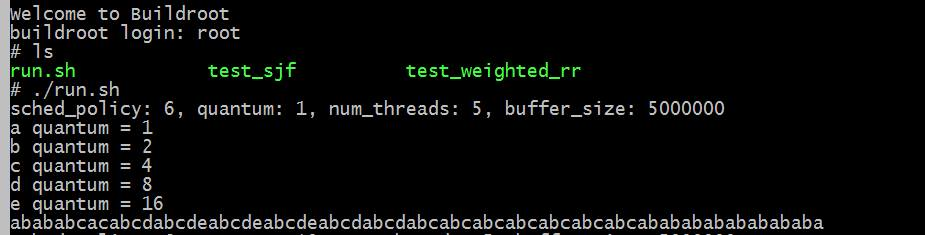
\includegraphics[width=400pt]{images/exp-weighted-rr.jpg}
        \caption{Weighted Round-Robin Scheduler 執行結果}
        \label{fig: result}
    \end{center}
\end{figure}

\begin{figure}[htp]
    \begin{center}
        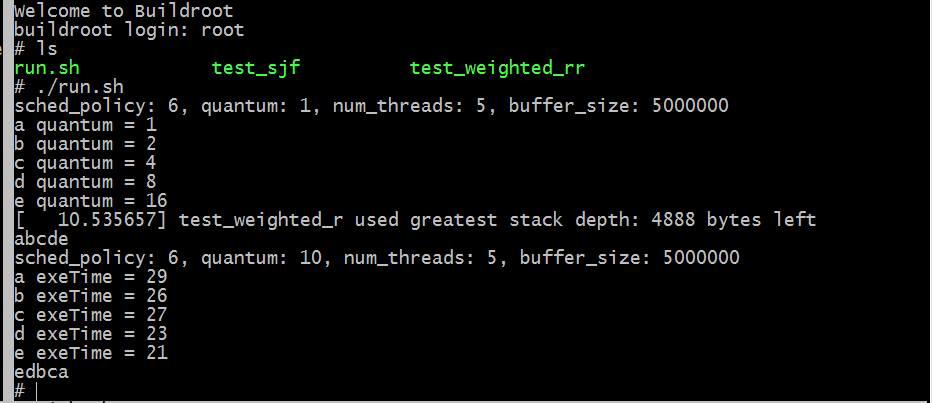
\includegraphics[width=400pt]{images/exp-sjf.jpg}
        \caption{Shortest Job First Scheduler 執行結果}
        \label{fig: result}
    \end{center}
\end{figure}

\vspace*{.1in} \noindent {\large \bfseries 附錄}

\end{resume}

\end{document}